\documentclass[a4paper,12pt]{article}
\usepackage{fontspec}
\usepackage{polyglossia}
\usepackage{csquotes}
\setdefaultlanguage[spelling=new, babelshorthands=true]{german}

% Seitenränder
\usepackage[left=2.5cm, right=2.5cm, head=1.25cm, bottom=2cm, foot=1.25cm, includefoot]{geometry}

% Fußzeile und Kopfzeile
\usepackage{fancyhdr}
\renewcommand{\headrulewidth}{0pt}
\renewcommand{\footrulewidth}{0.5pt}
\def \footer{
\begin{center}
\hfill
\fontsize{\footerFontSize}{\footerFontSize}\selectfont%\thesisFooterTitle
\hfill
\thepage
\end{center}
}

% Positioniert die Fußnoten fest am unteren Ende der Seite
\usepackage[bottom]{footmisc}

% Zeilenabstand: 1.5
\usepackage{setspace}
\setstretch{1.5}

\usepackage{graphicx}
\graphicspath{ {./images/} }

% Literaturverzeichnis
\usepackage[natbib=true, backend=biber, style=ieee]{biblatex}
\addbibresource{main.bib}

\begin{document}

% Titlepage
\begin{titlepage}

\title{Die Einkommensungleichheit in Deutschland seit der Wiedervereinigung}    

\author{Jona Rumberg}


\end{titlepage}

\maketitle
\thispagestyle{empty}
\newpage
\pagenumbering{arabic}

% Einleitung
\section*{Einleitung}
% Kurzer politischer Abriss
Die Einkommensungleichheit in Deutschland ist ein Thema von großer gesellschaftlicher und politischer Bedeutung. Insbesondere seit der Wiedervereinigung haben sich die wirtschaftlichen und sozialen Rahmenbedingungen in Ost- und Westdeutschland stark verändert. In dieser Arbeit wird ein Überblick über die Entwicklung der Einkommensungleichheit in Deutschland seit der Wiedervereinigung gegeben. Dabei werden verschiedene Aspekte wie die Entwicklung der Lorenzkurve, der Gini-Koeffizient und die Unterschiede zwischen West- und Ostdeutschland betrachtet. Das Ziel dieser Arbeit ist es, ein besseres Verständnis für die Einkommensverteilung in Deutschland zu gewinnen und mögliche Ursachen und Auswirkungen der Einkommensungleichheit zu analysieren.


% Hauptteil
\section*{Hauptteil}
\subsection*{Entwicklung der Lorenzkurve}
Mithilfe von Daten der Datenbank eurostat sollen im folgenden der Verlauf der Lorenzkurve analysiert werden. 
Die Lorenzkurve ist ein wichtiges Instrument zur Messung der Einkommensverteilung in einer Volkswirtschaft.
Sie stellt die kumulative Verteilung der Einkommen in einer Volkswirtschaft dar und ermöglicht es, die Einkommensverteilung zu grafisch darzustellen.
Die Entwicklung der Lorenzkurve in Deutschland seit der Wiedervereinigung wird anhand von Daten aus der Datenbank eurostat dargestellt.
Verglichen werden sollen dabei die Lorenzkurven für 1995, 2016 und 2022, um ein aussagekräftiges Bild der Entwicklung kurz nach der Wende, 20 Jahre danach und heute zu erhalten.

\begin{figure}[h]
\centering
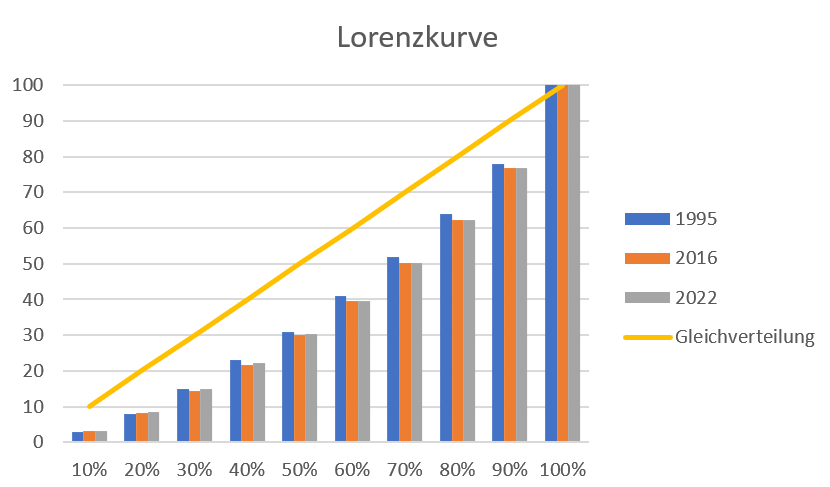
\includegraphics[width=1.0\textwidth]{Lorenzkurve.png}
\caption[short]{Lorenzkurven im Jahr 1995, 2016 und 2022 nach eigener Darstellung auf Basis von Daten der Datenbank eurostat \cite{eurostat_2024}}
\end{figure}

% Mittelschicht und untere Oberschicht leicht gesunken
% Unterschicht hat sich gehalten und sogar leicht verbessert

Zu sehen ist, dass sich die Lorenzkurve in den Jahren 1995, 2016 und 2022 nicht dramatisch verändert hat. Trotzdem ist eine leichte Entwicklung zu erkennen.
Die Dezil der Mittelschicht und die untere Oberschicht sind um ca. 2 Prozentpunkte nach unten verschoben. Interessanterweise hat sich dazu gegensätzlich die Unterschicht entwickelt.
Der Anteil am Gesamteinkommen ist hier im Vergleich der Jahre 1995 und 2022 um ca. 1 Prozentpunkt gestiegen. Insgesamt kann man sagen, dass die Ungleichheit in Deutschland gestiegen ist, die Unterschicht jedoch unterproportional
von dieser Entwicklung betroffen ist. Das in den Medien häufig prophezeite Ende der Mittelschicht und die im Allgemeinen steigende Ungleichheit bildet sich also gewissermaßen in den Daten ab. Konkrete politische und gesellschaftliche Gründe für diese Entwicklung nachzuvollziehen, 
würden den Rahmen dieser Arbeit sprenge, Faktoren könnten jedoch geopolitische Entwicklungen, demographischer Wandel oder weltwirtschaftliche Veränderungen sein.

\subsection*{Gini Koeffizient}


\begin{figure}[h]
\centering
\includegraphics*[width=1.0\textwidth]{gini}
\caption[short]{Gini Koeffizient in Deutschland. Darstellung durch WSI auf Basis von Daten des SOEP \cite{wsi_2024}}
\end{figure}

Als nächstes soll der Gini Koeffizient in seinem historischen Verlauf betrachtet werden. Der Gini Koeffizient quantifiziert die Ungleichheit in einer Volkswirtschaft und errechnet sich direkt aus der Lorenzkurve. In der Gesamtbetrachtung
ist erkennbar, dass die Ungleichheit in Deutschland seit der Wiedervereinigung gestiegen ist. Somit lässt sich die Erkenntnis, die aus der vorherigen Betrachtung der Lorenzkurve hervorgegangen ist verifizieren. Weiterhin ermöglicht es diese Betrachtung aber auch, 
die Entwicklung der Ungleichheit in einen historischen Kontext zu setzen. Vor allem in den frühen 2000er Jahren ist ein starker Anstieg zu erkennen. An dieser Stelle können wieder eine Vielzahl von Faktoren herangezogen werden, eine Veröffentlichung des DIW nennt beispielsweise
die ab um 2005 herum hohe Arbeitslosigkeit. \cite{grabka_goebel_2020}
Im Allgemeinen kann die Entwicklung in drei Phasen unterteilt werden:  \begin{itemize}
    \item 1994-98: ein leichter Rückgang der Einkommensungleichheit;
    \item 1995-2005: ein starker Anstieg;
    \item 2006-11: ein leichter Rückgang bei stagnierender bzw. leicht ansteigender Armutsgefährdung \cite{gebauer_martens_2020}
\end{itemize}
In der oben zitierten Veröffentlichung des BPB wird weiterhin auf den Zusammenhang zwischen der allgemeinen Einkommensentwicklung und der Einkommensungleichheit hingewiesen. So seinen eine Einkommenssteigerung in Kombination mit Veränderungen des Steuerrechts vor allem den oberen Einkommensgruppen zugute gekommen, was ein wesentlicher Faktor für die Steigerung der Ungleichheit sei. \cite{gebauer_martens_2020}

\subsection*{West und Ost}

Für die Arbeit interessant sind weiterhin die Entwicklungen in Ost- und Westdeutschland, die in der Grafik zusätzlich gegenübergestellt werden. Zu sehen ist, dass der Gini Koeffizient in Ostdeutschland durchgängig unter dem Wert für Westdeutschland liegt. Der Grund
hierfür ist dem WSI zufolge "das Erbe der deutlich egalitäreren Einkommensstruktur der DDR".\ \cite{wsi_2024} Damit gemeint ist, dass im Sozialismus systembedingt mit radikaleren Maßnahmen nach einer Gleichverteilung gestrebt wurde. So wurden beispielsweise in der Zeit der 
sowjetischen Besatzung Großgrundbesitzer enteignet und das Land an Kleinbauern verteilt (Bodenreform).
Das Ganze muss jedoch insofern kontextualisiert werden, als dass als weitere Folge des Sozialismus ein bis heute spürbares Einkommensgefälle zwischen Ost und West besteht. \cite{gebauer_martens_2020}
Es ist jedoch anzumerken, dass die Differenz zwischen Ost und West in den letzten Jahren abgenommen hat. Während der Gini Koeffizient für Ostdeutschland kurz nach der Wiedervereinigung noch ca. 0.05 Punkte unter dem Wert für Westdeutschland lag, ist dieser Unterschied heute auf ca. 0.03 Punkte gesunken.

\subsection*{Aktuelle Entwicklungen}
Die bisher zitierten Statistiken und Grafiken bezogen sich hauptsächlich auf historische Entwicklungen seit der Wiedervereinigung. Nun soll zum Abschluss der Betrachtungen zusätzlich ein Blick auf die aktuellen wirtschaftlichen Entwicklungen, vor allem mit Blick auf die Corona-Pandemie geworfen werden.
Die Pandemie ist ein, in jüngerer Vergangenheit beispielloses globales Ereignis, das auch in Deutschland zu tiefgreifenden Einschnitten in allen Lebensbereichen geführt hat. Eine Veröffentlichung des WSI zeigt, dass auch die Einkommensungleichheit in Deutschland von der Pandemie nicht unberührt geblieben sind. So sein Eine Untersuchung des WSI zeigt, "die unteren Einkommensgruppen Einbußen erlitten haben."\ \cite{kohlrausch_zucco_hövermann_2020} Das lege nahe, dass die Ungleichheit weiter gestiegen sein könne. In der Veröffentlichung des WSI wird weiterhin analysiert, dass vor allem Personen mit sowieso geringem Einkommen, Selbstständige, Eltern und Personen mit Migrationshintergrund überproportional von den wirtschaftlichen Folgen der Pandemie betroffen sind. Auch Kurzarbeit haben vor allem Personen aus diesen Gruppen in überdurchschnittlichem Ausmaß in Anspruch nehmen müssen. \cite{kohlrausch_zucco_hövermann_2020}


% Fazit

\section*{Fazit}

In der Arbeit wurde die Entwicklung der Einkommensungleichheit in Deutschland seit der Wiedervereinigung skizziert. Dabei wurde festgestellt, dass die Ungleichheit in Deutschland seit der Wiedervereinigung gestiegen ist und das Ganze mit verschiedenen Instrumenten belegt werden. Relevante Teilaspekte der Betrachtung sind die Unterschiede zwischen Ost und West und wie abschließend bei der Betrachtung der aktuellen Entwicklungen kurz angerissen, die Betrachtung verschiedener sozialer Gruppen.

Die gesellschaftliche und politische Bedeutung dieser Entwicklung ist enorm. Die Einkommensungleichheit hat Auswirkungen auf das soziale Gefüge einer Gesellschaft und kann zu sozialen Spannungen führen. Eine politische Bearbeitung der Thematik ist somit unabdingbar. Wie am Beispiel der Corona-Pandemie gezeigt, haben neben gesamtwirtschaftlichen Entwicklungen vor allem Krisen einen Einfluss auf die Einkommensverteilung. Es ist also zu erwarten , dass mit Blick auf die Zukunft die Einkommensungleichheit weiterhin ein wichtiges Thema bleiben wird und in der öffentlichen Debatte eine wichtige Rolle spielen wird.







% Literaturverzeichnis
\newpage
\setstretch{1.0}
\printbibliography
\thispagestyle{empty}

\end{document}